\documentclass[12pt,onecolumn,a4paper,fleqn]{article}
\usepackage[top=1in, bottom=1in, left=0.75in, right=0.75in]{geometry}
\usepackage{epsfig,graphicx,subfigure,amsthm,amsmath}
\usepackage[table,xcdraw,svgnames]{xcolor}
\usepackage{setspace}
\usepackage{mathtools}
\usepackage{fancyhdr}
\usepackage{sidecap}
\usepackage{tikz}
\usepackage{pgfplots}
\usetikzlibrary{decorations.pathreplacing}
\usepackage{relsize}
\usepackage{color,xcolor}
\usepackage[framed,numbered]{matlab-prettifier}
\usepackage{float}
\usepackage{enumerate}
\usepackage{booktabs}
\usepackage{setspace}
\usepackage{datetime}
\usepackage{xepersian}


\settextfont[Path=fonts/,BoldFont={ZarBd.ttf},BoldFeatures={Scale=0.9}]{BZar.ttf}

%\DeclarePairedDelimiter\ceil{\lceil}{\rceil}
%\DeclarePairedDelimiter\floor{\lfloor}{\rfloor}

\definecolor{vgreen}{RGB}{104,180,104}
\definecolor{vblue}{RGB}{49,49,255}
\definecolor{vorange}{RGB}{255,143,102}

\pagestyle{fancy}
\fancyhf{}
\rhead{\textbf{آزمایشگاه طراحی سیستم‌های دیجیتال}}
\chead{\textbf{گزارش آزمایش سوم}}
\lhead{\textbf{\nouppercase{\rightmark}}}
\cfoot{({\thepage})}
\renewcommand{\headrulewidth}{1pt}
\renewcommand{\footrulewidth}{1pt}
\renewcommand{\sectionmark}[1]{\markright{#1}}
\renewcommand{\subsectionmark}[1]{\markright{#1}}
%\newdateformat{monthyeardate}{%
%	\monthname[\THEMONTH], \THEYEAR}

\onehalfspacing
\begin{document}
	%%% title pages
	\large
	\begin{titlepage}
		
		\begin{center}
			\begin{huge}
				\textbf{
					به نام خدا\\
				}
			\end{huge}
			
			\vspace*{1.5cm}
			
\includegraphics[scale=0.9]{source/sharif_logo.png}\\
			\vspace*{0.5cm}
			\begin{Large}
				
				دانشگاه صنعتی شریف\\
				\vspace*{0.25cm}
				\textbf{
					دانشکده مهندسی کامپیوتر\\
				}
			\end{Large}
			\vspace*{3cm}
			\begin{huge}
				\textbf{
					آزمایشگاه طراحی سیستم‌های دیجیتال\\
					\vspace*{1.75cm}
				}
			\end{huge}
			
			\begin{Large}
				\textbf{
					آزمایش سوم:\\
					طراحی مقایسه‌کننده باینری به صورت ترکیبی و ترتیبی\\
				}
			\end{Large}
			
			\noindent\rule[1ex]{\linewidth}{1pt}
			\vspace*{1.5cm}
			\begin{Large}
				محمدجواد هزاره، یاسین موسوی
				
				\vspace*{1.5cm}
				%					\textbf{\today}
				\textbf{
					تابستان 1400
				}
			\end{Large}			
		\end{center}
		\thispagestyle{empty}
	\end{titlepage}	
	\pagebreak
	
	\tableofcontents
	\thispagestyle{empty}
	\pagebreak
	\section{مقدمه}
	\subsection{شرح آزمایش}
	در این آزمایش هدف طراحی یک مقايسه‌کننده باینری هم به صورت ترکیبی و هم به صورت ترتیبی است. طراجی با استفاده از زبان
	\lr{verilog}
	 و به شکل توصیف جریان داده صورت گرفته است.
	\pagebreak
	\section{مدار ترکیبی}
	\subsection{رابط‌ کاربری}
	رابط کاربری مدار ترکیبی بسیار ساده بوده و شامل دو ورودی چهار بیتی
	\lr{A}
	و
	\lr{B}
	می‌شود. خروجی مدار نیز سه سیگنال 
	\lr{eq}،
	\lr{gt}
	و
	\lr{lt}
	را در بر می‌گیرد که فعال خواهند بود اگر به ترتیب ورودی‌ها با یکدیگر برابر باشند، یا ورودی 
	\lr{A}
	بزرگ‌تر از ورودی 
	\lr{B}
	باشد و یا ورودی
	\lr{A}
	کوچک‌تر از ورودی 
	\lr{B}
	باشد.
	\begin{figure}[H]
		\centering
		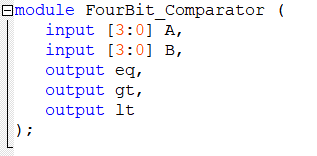
\includegraphics[scale=0.95]{source/interface_comb.png}
		\caption{رابط کاربری مدار ترکیبی}
	\end{figure}
	\subsection{نحوه کار}
	برای پیاده‌سازی مدار، از واحد مقايسه‌کننده یک بیتی استفاده شده و چهار عدد از این مقايسه‌کننده‌ها پشت‌سر یکدیگر استفاده شده‌اند. به این صورت که اول بیت های با ارزش بالاتر مقایسه می‌شوند و سپس به سراغ بیت‌های با ارزش کم‌تر رفته و نتیجه مقایسه بیت‌های قبلی را با خود به این مرحله می‌آوریم. این مقایسه‌کننده یک بیتی به این صورت رفتار می‌کند که علاوه بر دو ورودی‌ای که برای بیت‌های مقایسه‌شونده می‌گیرد، سه ورودی دیگر نیز می‌گیرد که نتیجه مقایسه بیت‌های با ارزش بالاتر دو عدد اصلی هستند. خروجی آن نیز سه سیگنال
	\lr{eq}،
	\lr{gt}
	و
	\lr{lt}
	هستند که نتیجه مقایسه اعداد مدنظر با احتساب یک بیت جدید می‌باشند.
	\subsection{شبیه‌سازی}
	نتیجه شبیه‌سازی مدار مورد نظر در شکل \ref{fig:sim_comb} آورده شده است.
	\begin{figure}[H]
	\centering
	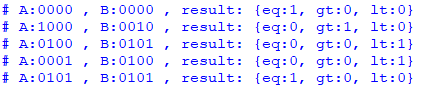
\includegraphics[scale=1.2]{source/sim_comb.png}
	\caption{نتیجه شبیه‌سازی مدار ترکیبی}
	\label{fig:sim_comb}
	\end{figure}
	\pagebreak
	\section{مدار ترتیبی}
	\subsection{رابط کاربری}
	رابط کاربری مدار ترتیبی دو ورودی تک بیتی 
	\lr{a}
	و
	\lr{b}
	که بیت‌های عدد ورودی می‌باشند
	و همچنین ورودی‌های 
	\lr{clk}
	و
	\lr{reset}
	هستند. خروجی‌های آن نیز به طور مشابه
	\lr{eq}،
	\lr{gt}
	و
	\lr{lt}
	بوده که نتیجه مقایسه تا بیت حال حاضر را نشان می‌دهند.
	\begin{figure}[H]
		\centering
		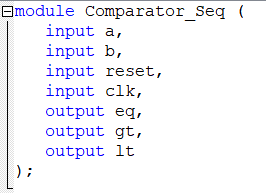
\includegraphics[scale=0.95]{source/interface_seq.png}
		\caption{رابط کاربری مدار ترتیبی}
	\end{figure}
	\subsection{نحوه کار}
	نحوه کار این مدار برخلاف مدار ترکیبی، به این صورت است که نخست بیت‌های با ارزش پایین بررسی می‌شوند و نتیحه در یک فلیپ‌فلاپ ذخیره شده و هنگام بررسی بیت‌های با ارزش بالاتر از این نتیجه استفاده می‌شود.
	\subsection{شبیه‌سازی}
	نتیجه شبیه‌سازی این مدار نیز در شکل \ref{fig:sim_seq} آورده شده است.
	\begin{figure}[H]
		\centering
		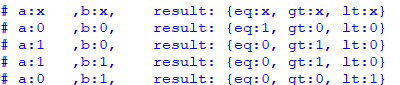
\includegraphics[scale=1.2]{source/sim_seq.png}
		\caption{نتیجه شبیه‌سازی مدار ترتیبی}
		\label{fig:sim_seq}
	\end{figure}
\end{document}